\documentclass[a4paper,10pt]{article}

% рисунки
\usepackage{graphicx}

\usepackage[T2A]{fontenc}
\usepackage[utf8]{inputenc}
\usepackage[english,russian]{babel}

\RequirePackage{caption}
\DeclareCaptionLabelSeparator{defffis}{ — }
\captionsetup{justification=centering,labelsep=defffis}

\usepackage{caption} \captionsetup[table]{labelsep=endash,justification=justified,singlelinecheck=false,font=normalsize}

\usepackage{amsmath,amsfonts,amssymb,amsthm,mathtools}



\begin{document}
  
\begin{center}
  \section*{Лабораторная работа №3.5.1 \\Изучение плазмы газового разряда в неоне\\Джокер Бэтмен, Б02-000, 25.09.2021}
\end{center}  

\vspace{5mm}
\section*{Введение}

\begin{flushleft}
  \textbf{Цель работы:} изучение вольт-амперной характеристики тлеющего разряда; изучение свойств плазмы методом зондовых характеристик.
\end{flushleft}

\begin{flushleft}
  \textbf{В работе используются:} стеклянная газоразрядная трубка, наполненная неоном, высоковольтный источник питания, источник питания постоянного тока, делитель напряжения, резистор, потенциометр, амперметры, вольтметры, переключатели.
\end{flushleft}

\section*{Теоретическая справка}

\textit{Двойным зондом} назывется система, состоящая их двух одинаковых зондов, расположенных на небольшом расстоянии друг от друга. Между зондами создаётся разность потенциалов $U$, которая по велиине много меньше плавающего потенциала: $\left|U\right|\ll\left|U_f\right|$. При этом оба зонда имеют относительно плазмы близкий к плавающему отрицательный потенциал, т.е. находятся на \textit{ионной} ветви вольт-амперной характеристики.

При отсутствии разности потенциалов ток между зондами равен нулю. Рассчитаем величину тока, проходящего через двойной зонд вблизи точки $I=0$. При небольших разностях потенциалов ионные токи на оба зонда равны ионному току насыщения и компенсируют друг друга. Величина результирующего тока целиком связана с различием в электронных токах. Пусть потенциал на первом зонде равен\[U_1=U_f+\Delta U_1,\]а на втором\[U_2=U_f+\Delta U_2.\]Предполагается, что $\Delta U_1,\Delta U_2\ll U_f$. Напряжение $U$ между зондами равно\[U=U_2-U_1=\Delta U_2-\Delta U_1.\]

Найдём ток, приходящий на первый электрод:\[I_1=I_{i\text{н}}-I_{e0}\exp{\left(\frac{eU_1}{k_{\text{Б}T_e}}\right)}=I_{i\text{н}}-\left[I_{e0}\exp{\left(\frac{eU_f}{k_{\text{Б}T_e}}\right)}\right]\exp{\left(\frac{e\Delta U_1}{k_{\text{Б}T_e}}\right)}.\]Заметим, что при $\Delta U_1=0$ (при $U_1=U_f$) электронный и ионный ток компенсируют друг друга. Это означает, что заключённый в квадратные скобки множитель равен $I_{i\text{н}}$. Имеем поэтому\[I_1=I_{i\text{н}}\left[1-\exp{\left(\frac{e\Delta U_1}{k_{\text{Б}T_e}}\right)}\right].\]Аналогично для второго электрода\[I_2=I_{i\text{н}}\left[1-\exp{\left(\frac{e\Delta U_2}{k_{\text{Б}T_e}}\right)}\right].\]

Заметим, что зонды 1 и 2 соединены \textit{последовательно} -- через плазму -- поэтому $I_1=-I_2=I$. Выразим $\Delta U_1$ и $\Delta U_2$ из уравнений выше:\[\Delta U_1=\frac{k_{\text{Б}}T_e}{e}\ln{\left(1-\frac{I}{I_{i\text{н}}}\right)},\ \Delta U_2=\frac{k_{\text{Б}}T_e}{e}\ln{\left(1+\frac{I}{I_{i\text{н}}}\right)}.\]Наконец, вычитая второе равенство из первого, найдём\[U=\Delta U_1-\Delta U_2=\frac{k_{\text{Б}}T_e}{e}\ln{\left(\frac{I_{i\text{н}}-I}{I_{i\text{н}}+I}\right)},\]и, разрешая это равенство относительно $I$, получим\[I=I_{i\text{н}}\th{\frac{eU}{2k_{\text{Б}}T_e}}.\]Эту формулу можно использовать для определния температуры электронов по форме вольт-амперной характеристики двойного зонда.

Наблюдаемая на опыте зависимость тока от напряжения изображена на рисунке \Ref{Tok}. Заметим, что эта кривая отличается от теоретической существованием наклона у асимптот в области больших $\left|U\right|$, что связано с ускорением частиц плазмы приложенным полем, которое не учтено при выводе теоретической зависимости.

Графики типа \Ref{Tok} проще всего обрабатывать следующим образом. Сначала находится ток насыщения $I_{i\text{н}}$ из пересечения асимптот с осью $U=0$. Затем находится наклон графика в начале координат, из которого можно определить температуру электронов $T_e$. Дифференциируя формулу для $I$ по $U$ в точке $U=0$ и принимая во внимание, что при малых аргументах $\th{x}\approx x$, найдём\[k_{\text{Б}}T_e=\frac{1}{2}\frac{eI_{i\text{н}}}{\frac{\text{d}I}{\text{d}U}\vert{}_{U=0}},\]где $\frac{\text{d}I}{\text{d}U}\vert{}_{U=0}$ -- наклон характеристики зонда вблизи начала координат. По известным $T_e$ и $I_{i\text{н}}$ можно найти концентрацию заряженных частиц $n_i=n_e$.

Таким образом, двойные зонды удобно применять для измерения электронной температуры и концентрации частиц в плазме.

\begin{figure}[h]
	\centering
	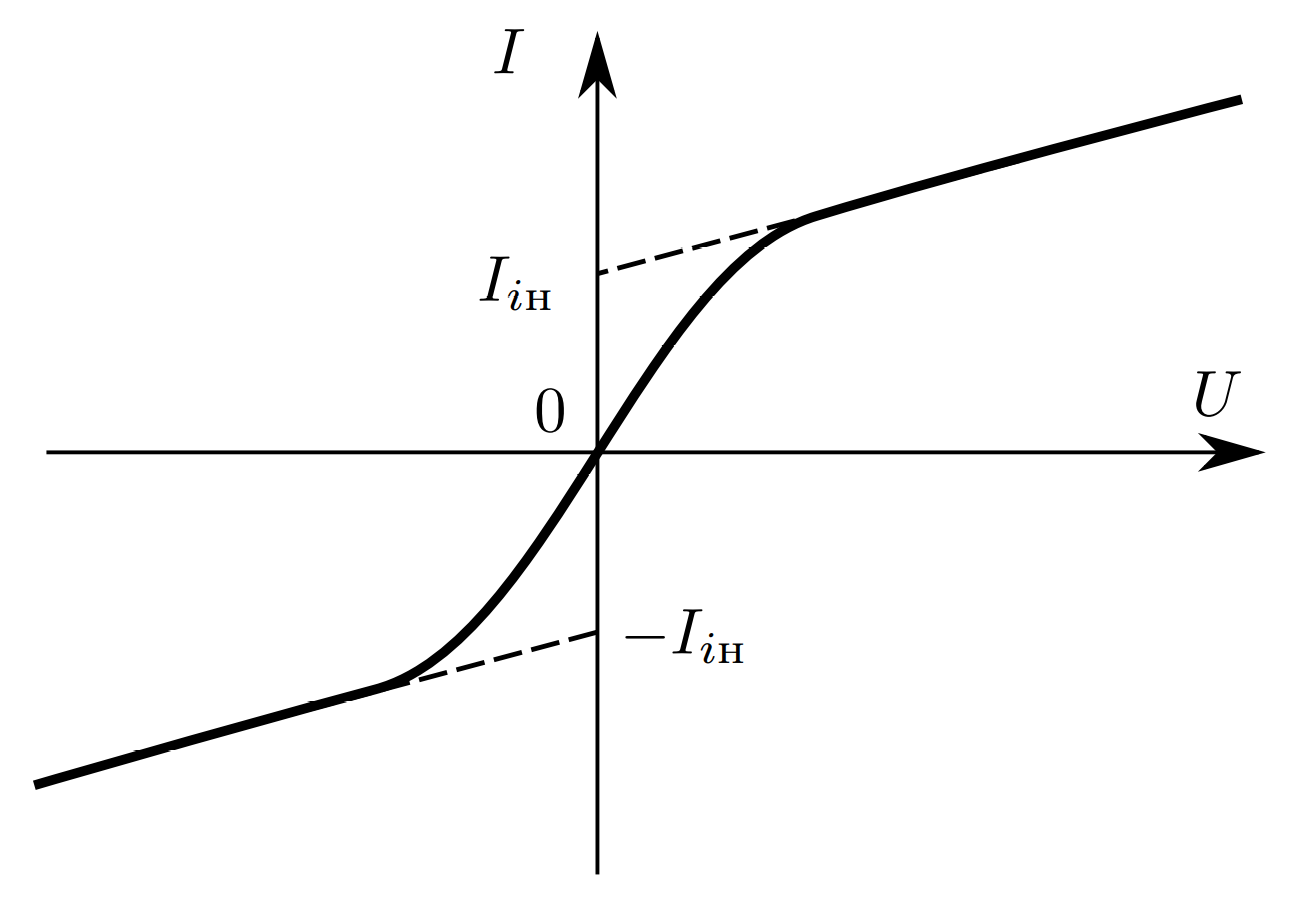
\includegraphics[scale=0.30]{Tok}
	\caption{Вольт-амперная характеристика двойного зонда} \label{Tok}
\end{figure}

\section*{Экспериментальная установка}

Схема установки для исследования плазмы газового разряда в неоне представлена на рисунке \Ref{Device}. Стеклянная газоразрядная трубка имеет холодный (ненагреваемый) полый катод, три анода и \textit{геттерный узел} -- стеклянный балон, на внутреннюю поверхность которого напылена газопоглощающая плёнка (\textit{геттер}). Трубка наполнена изотопом неона ${}^{22}\text{Ne}$ при давлении 2 мм рт. ст. Катод и один из анодов (I или II) с помощью переключателя $\text{П}_1$ подключаются через балластный резистор $R_{\text{б}}$ ($\sim450~\text{к}\Omega$) к регулируемому высоковольтному источнику питания (ВИП) с выходным напряжением до 5 кВ.

\begin{figure}[h]
	\centering
	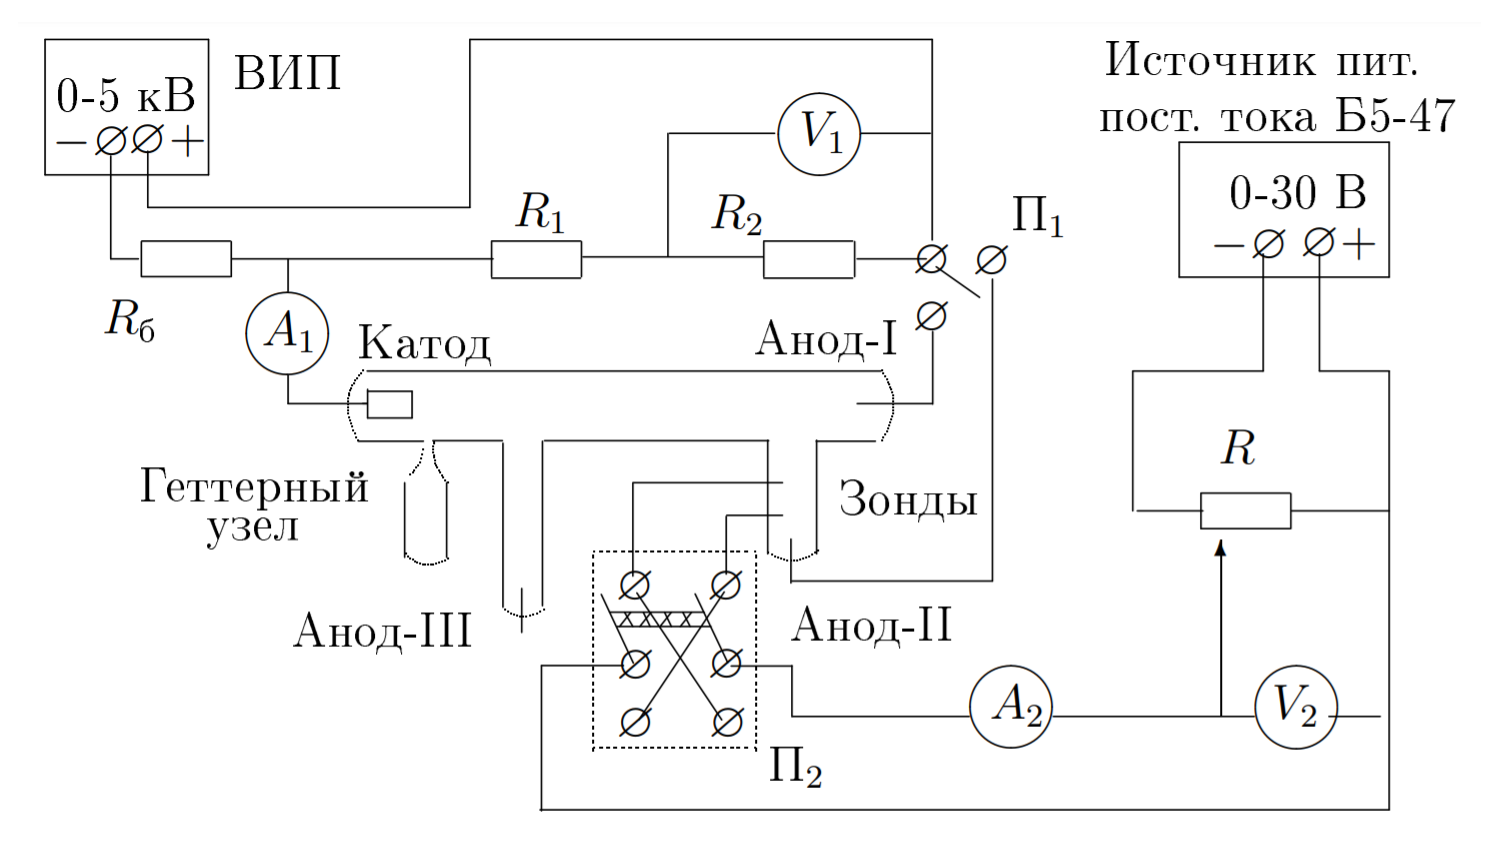
\includegraphics[scale=0.30]{Device}
	\caption{Схема установки для исследования газового разряда} \label{Device}
\end{figure}

При подключении к ВИП анода-I между ним и катодом возникает газовый разряд. Ток разряда измеряется миллиамперметром $A_1$, а падение напряжение на разрядной трубке -- цифровым вольтметром $V_1$ (мультиметром GDM), подключённым к трубке через высоомный ($25~\text{М}\Omega$) делитель напряжения с коэффициентом $\frac{R_1+R_2}{R_2}=10$.

При подключении к ВИП анода-II разряд возникает в пространстве между катодом и анодом-II, где находится двойной зонд, используемый для диагностики плазмы положительного столба.

Зонды изготовлены из молибденовой проволоки диаметром $d=0,2~\text{мм}$ и имеют длину $l=5,2~\text{мм}$. Они подключены к источнику питания GPS через потенциометр $R$. Переключатель $\text{П}_2$ позволяет изменять полярность напряжения на зондах. Величина напряжения на зондах изменяется с помощью дискретного переключателя "$V$" выходного напряжения источника питания и потециометра $R$, а измеряется цифровым вольтметром $V_2$ (GMD). Для измерения зондового тока используется мультиметр $A_2$ (GDM). Анод-III в нашей работе не используется.

\section*{Ход работы}

\section*{I. Вольт-амперная характеристика разряда}

Подготовим все приборы к работе. Включим в сеть ВИП и мультиметр $V_1$. Будем плавно увеличивать выходное напряжение ВИП с нулевого значения до того момента, как в трубке зажжётся разряд. Показания вольтметра $V_1$ непосредственно перед зажиганием -- т.н. напряжение зажигания разряда -- равны $U_{\text{заж}}=\left(231\pm3\right)~\text{В}$.

С помощью вольтметра $V_1$ и амперметра $A_1$ снимем вольт-амперную характеристику разряда $U_{\text{р}}\left(I_{\text{р}}\right)$ в диапазоне от $0,5~\text{мА}$ до $\approx5~\text{мА}$ по току. Измерения проведём как при нарастании ($\nearrow$), так и при убывании ($\searrow$) тока. Занесём полученные данные в таблицу \Ref{VAH}. Заметим заранее, что гистерезиса ВАХ в работе не наблюдается, поэтому при построении графика имеет смысл использовать значения, полученные при усреднении ($\langle\ldots\rangle$) снятых значений. Тоже занесём эти точки в таблицу.

Оценим также погрешности. Погрешность амперметра $A_1$ равна половине цены его деления, $\Delta I=0,02~\text{мА}$. Погрешность вольтметра равна $0,003U+4~\text{ед. мл. разряда}$.

\begin{table}[h]
	\centering
	\caption{Зависимость напряжения разряда $U_{\text{р}}$ от его тока $I_{\text{р}}$ при нарастании и убывании последнего} \label{VAH}
	\begin{tabular}{|c|c|c|c|c|c|c|c|c|}
		\hline
		$I_{\text{р}}$, мА & 0,60 & 0,80 & 1,00 & 1,20 & 1,40 & 1,60 & 1,80 & 2,00 \\ \hline
		$U_{\text{р}}^{\nearrow}$, В & 35,0 & 34,2 & 32,9 & 30,0 & 28,1 & 27,0 & 26,4 & 25,8 \\ \hline
		$U_{\text{р}}^{\searrow}$, В & 35,0 & 34,3 & 32,8 & 30,2 & 28,1 & 27,1 & 26,3 & 25,8 \\ \hline
		$U_{\text{р}}^{\langle\ldots\rangle}$, В & 35,0 & 34,3 & 32,9 & 30,1 & 28,1 & 27,1 & 26,4 & 25,8 \\ \hline
		\hline
		$I_{\text{р}}$, мА & 2,20 & 2,40 & 2,60 & 2,80 & 3,00 & 3,20 & 3,40 & 3,60 \\ \hline
		$U_{\text{р}}^{\nearrow}$, В & 25,3 & 25,2 & 24,8 & 24,6 & 24,3 & 24,1 & 24,1 & 24,0  \\ \hline
		$U_{\text{р}}^{\searrow}$, В & 25,4 & 25,0 & 24,8 & 24,6 & 24,2 & 24,0 & 24,0 & 24,0  \\ \hline
		$U_{\text{р}}^{\langle\ldots\rangle}$, В & 25,4 & 25,1 & 24,8 & 24,6 & 24,3 & 24,1 & 24,1 & 24,0 \\ \hline
		\hline
		$I_{\text{р}}$, мА & 3,80 & 4,00 & 4,20 & 4,40 & 4,60 & 4,80 & 5,00 & -- \\ \hline
		$U_{\text{р}}^{\nearrow}$, В & 24,0 & 23,9 & 23,8 & 23,8 & 23,7 & 23,7 & 23,6 & -- \\ \hline
		$U_{\text{р}}^{\searrow}$, В & 24,0 & 23,9 & 23,8 & 23,8 & 23,7 & 23,7 & 23,6 & -- \\ \hline
		$U_{\text{р}}^{\langle\ldots\rangle}$, В & 24,0 & 23,9 & 23,8 & 23,8 & 23,7 & 23,7 & 23,6 & -- \\ \hline
	\end{tabular}
\end{table}

Построим вольт-амперную характеристику разряда в координатах $I_{\text{р}}\left(U_{\text{р}}\right)$. Она представлена на рисунке \Ref{Zond_VAH}. По наклону кривой на левом конце графика определим минимальное дифференциальное сопротивление разряда $R_{\text{диф}}\equiv\frac{\text{d}U}{\text{d}I}=\left(-255\pm10\right)~\Omega$. Сравнив график с рисунком \Ref{Characteristic} (в Приложении к отчёту), сделаем вывод, что полученный в работе график \textit{соответствует участку Г--Д}.

\begin{figure}[h]
	\centering
	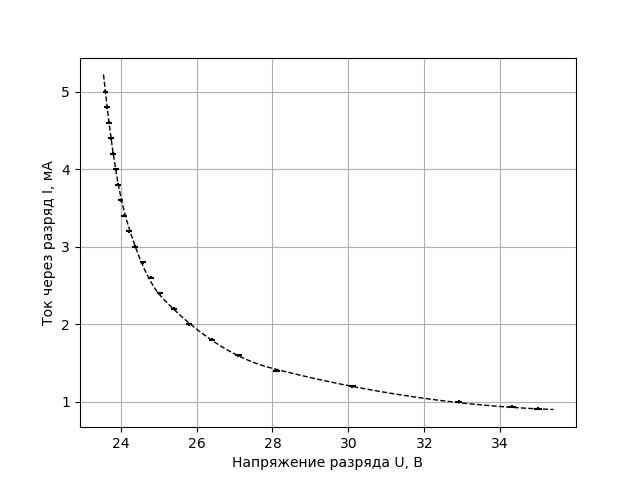
\includegraphics[scale=0.70]{Zond_VAH}
	\caption{Вольт-амперная характеристика разряда $I_{\text{р}}\left(U_{\text{р}}\right)$. Сглаживающая кривая проведена с помощью кубического сплайна} \label{Zond_VAH}
\end{figure}

\subsection*{II. Зондовые характеристики}

Подготовим приборы к работе. Плавно увеличивим напряжение ВИП до возникновения разряда. Установим максимально допустимое значение разрядного тока $I_{\text{р}}^{max}=5,0~\text{мА}$. Подготовим к работе источник питания, после чего с помощью потенциометра $R$ установим на зонда максимально допустимое напряжение $U_{\text{з}}^{max}=25,0~\text{В}$.

Измерим вольт-амперную характеристику двойного зонда $I_{\text{з}}\left(U_{\text{з}}\right)$ в диапазоне от $-U^{max}_{\text{з}}$ до $U^{max}_{\text{з}}$ при фиксированном токе разряда $I_{\text{р}}$. Проведём данные измерения при трёх различных значениях тока разряда ($1,5~\text{мА}$, $3,0~\text{мА}$ и $5,0~\text{мА}$ в таблице соответственно). Занесём полученные данные в таблицу \Ref{Holl}. Отцентрируем кривую: проведём ось абсцисс на уровне $I=\frac{1}{2}\sum\Delta I$ и восстановим ось ординат из точки пересечения кривой с осью абсцисс. Пересчитанные для этого точки с индексом $c$ также занесём в таблицу.

\begin{table}[h]
	\centering
	\caption{Зависимость напряжения на зонде $U_{\text{з}}$ от тока $I_{\text{з}}$ через него значениях $I_{\text{р}}=1,5~\text{мА},\ 3,0~\text{мА}\ \text{и}\ 5,0~\text{мА}$ соответственно} \label{Holl}
	\begin{tabular}{|c|c|c|c|c|c|c|c|c|c|}
		\hline
		$U_{\text{з}},\text{В}$ && $I_{\text{з}},\text{мкА}$ & $I_{\text{з}c},\text{мкА}$ && $I_{\text{з}},\text{мкА}$ & $I_{\text{з}c},\text{мкА}$ && $I_{\text{з}},\text{мкА}$ & $I_{\text{з}c},\text{мкА}$ \\ \hline
		25,0 && 39,8 & 37,1 && 77,8 & 73,3 && 124,0 & 118,0 \\ \hline
		22,0 && 38,4 & 35,7 && 75,6 & 71,1 && 127,1 & 121,1 \\ \hline
		19,0 && 37,1 & 34,4 && 73,4 & 68,9 && 125,4 & 119,4 \\ \hline
		16,0 && 35,8 & 33,1 && 70,1 & 65,6 && 121,4 & 115,4 \\ \hline
		13,0 && 34,1 & 31,4 && 67,2 & 62,7 && 113,1 & 107,1 \\ \hline
		10,0 && 31,1 & 28,4 && 60,5 & 56,0 && 99,4 & 93,4 \\ \hline
		8,0 && 27,9 & 25,2 && 53,6 & 49,1 && 86,4 & 80,4 \\ \hline
		6,0 && 23,4 & 20,7 && 44,5 & 40,0 && 69,9 & 63,9 \\ \hline
		4,0 && 17,5 & 14,8 && 32,4 & 27,9 && 49,2 & 43,2 \\ \hline
		2,0 && 10,1 & 7,4 && 18,3 & 13,8 && 24,9 & 18,9 \\ \hline
		0,0 && 2,7 & 0,0 && 4,5 & 0,0 && 6,0 & 0,0 \\ \hline
		-2,0 && -5,6 & -8,3 && -9,9 & -14,4 && -12,5 & -18,5 \\ \hline
		-4,0 && -12,9 & -15,6 && -24,0 & -28,5 && -36,8 & -42,8 \\ \hline
		-6,0 && -18,7 & -21,4 && -35,7 & -40,2 && -57,6 & -63,6 \\ \hline
		-8,0 && -23,0 & -25,7 && -44,9 & -49,4 && -74,8 & -80,8 \\ \hline
		-10,0 && -25,9 & -28,6 && -51,6 & -56,1 && -87,8 & -93,8 \\ \hline
		-13,0 && -28,6 & -31,3 && -57,9 & -62,4 && -101,4 & -107,4 \\ \hline
		-16,0 && -30,1 & -32,8 && -61,4 & -66,1 && -109,4 & -115,4 \\ \hline
		-19,0 && -31,2 & -33,9 && -63,7 & -68,2 && -113,1 & -119,1 \\ \hline
		-22,0 && -32,4 & -35,1 && -65,7 & -70,2 && -114,8 & -120,8 \\ \hline
		-25,0 && -33,5 & -36,2 && -67,7 & -72,2 && -112,2 & -118,2 \\ \hline
	\end{tabular}
\end{table}

Параметры используемого в работе зонда $d=0,2~\text{мм}$ и $l=5,2~\text{мм}$.

Построим теперь в отдельных системах координат отцентрированные зондовые характеристики для разных токов. Результаты построений приведены на рисунках \Ref{zoond1}, \Ref{zoond2} и \Ref{zoond3}.

\begin{figure}[h]
	\centering
	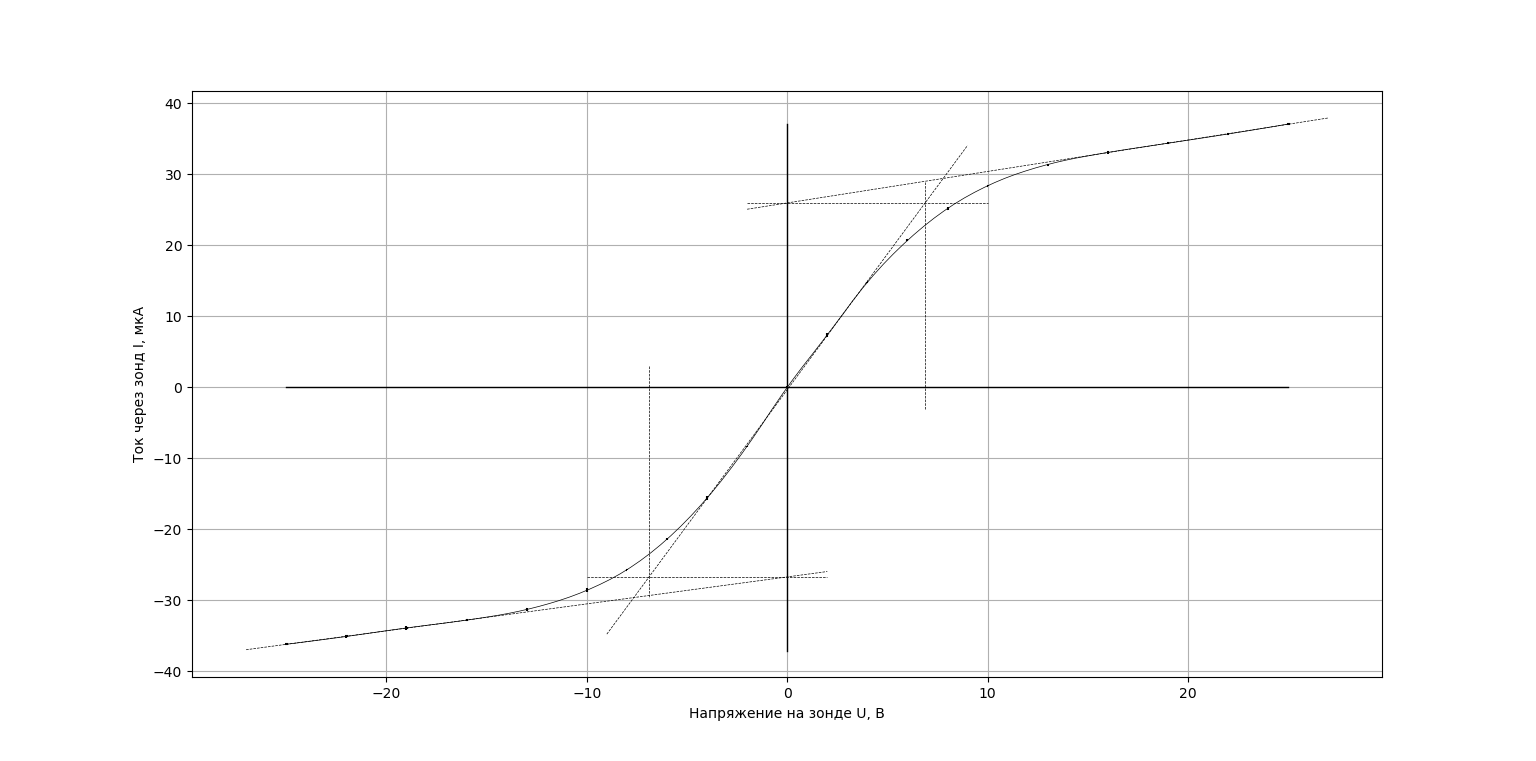
\includegraphics[scale=0.28]{zoond1}
	\caption{Зондовая характеристика $I_{\text{з}}\left(U_{\text{з}}\right)$ при токе через разряд $I_{\text{р}}=1,5~\text{мА}$. Сглаживающая кривая проведена с помощью кубического сплайна} \label{zoond1}
	\centering
	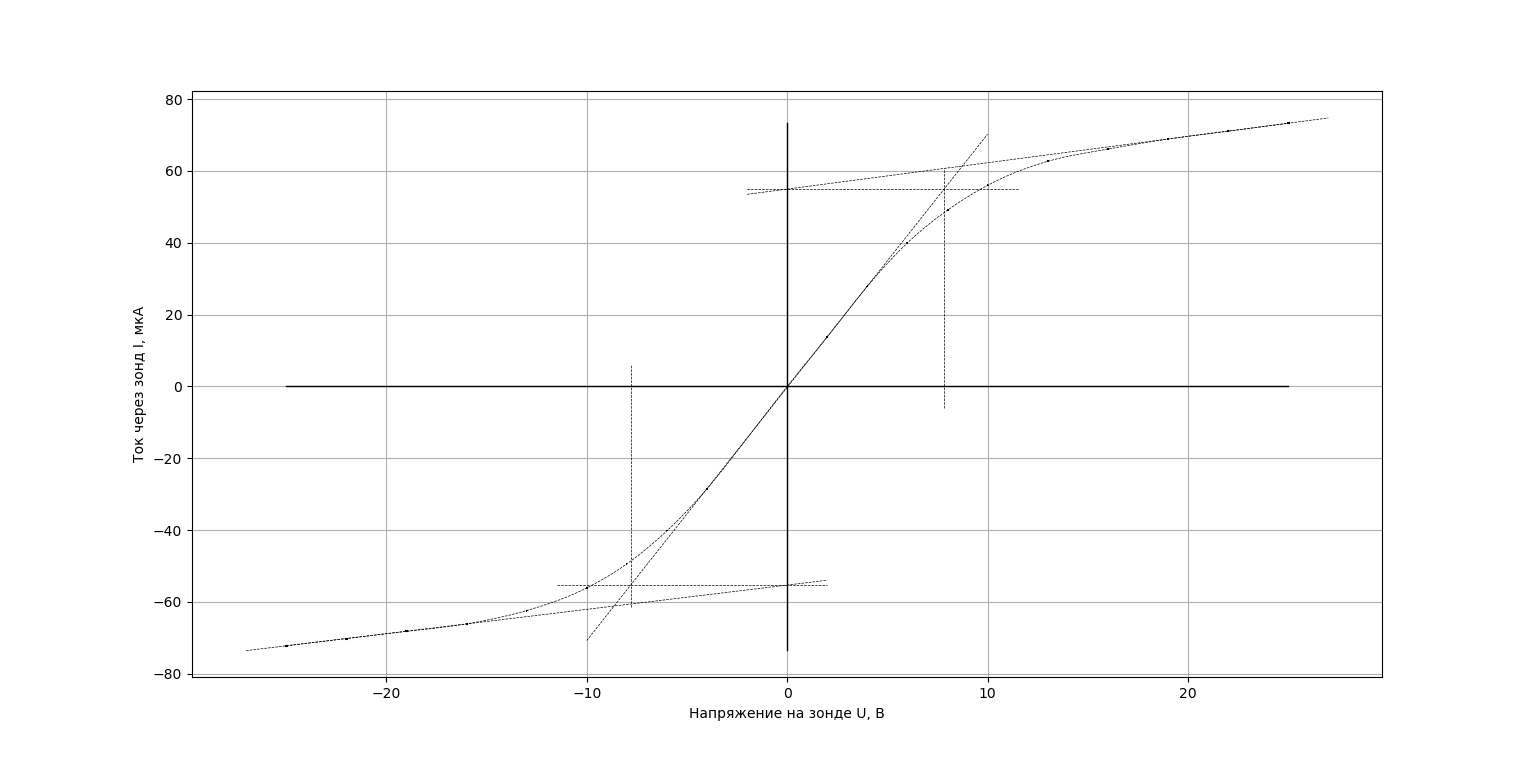
\includegraphics[scale=0.28]{zoond2}
	\caption{Зондовая характеристика $I_{\text{з}}\left(U_{\text{з}}\right)$ при токе через разряд $I_{\text{р}}=3,0~\text{мА}$. Сглаживающая кривая проведена с помощью кубического сплайна} \label{zoond2}
	\centering
	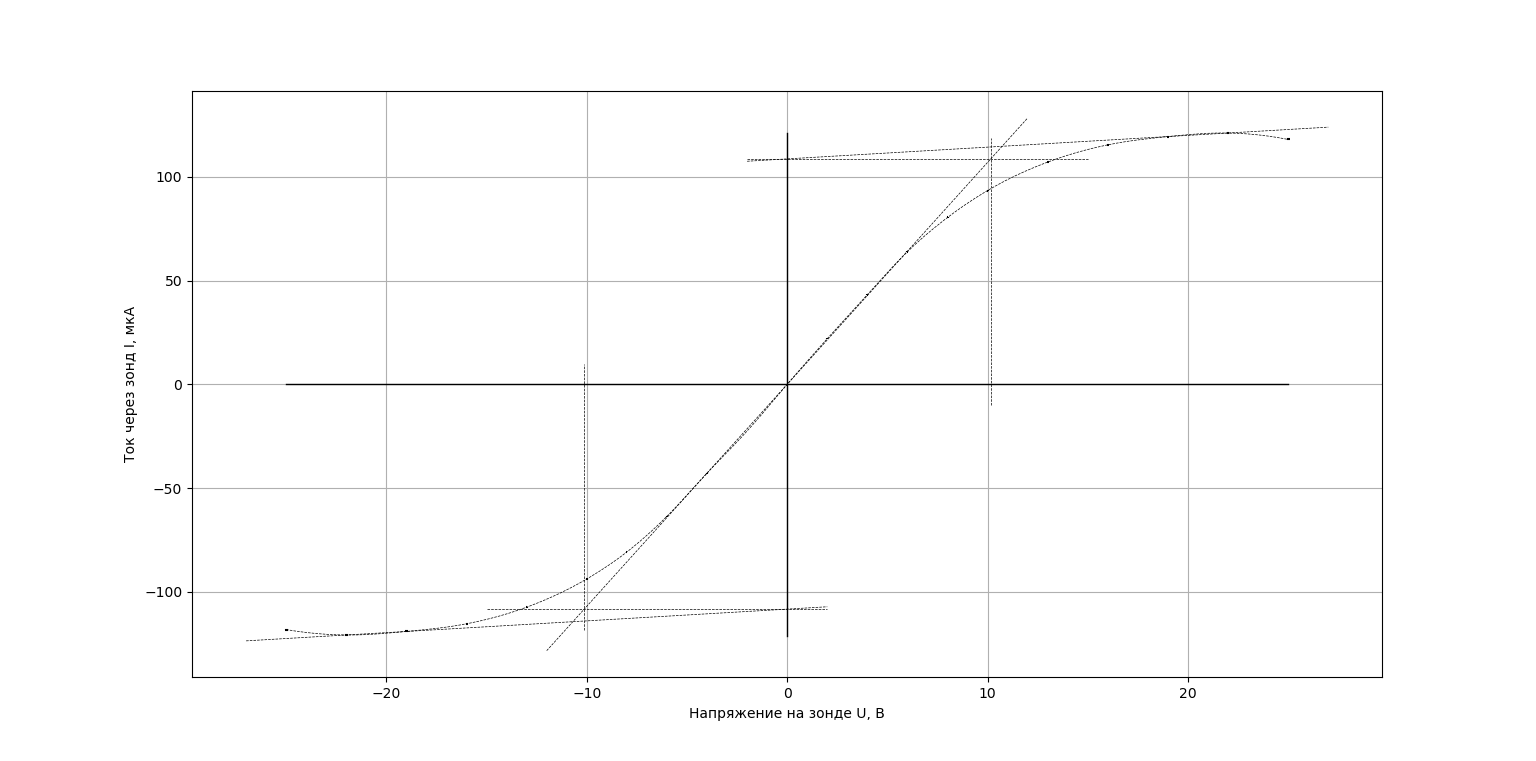
\includegraphics[scale=0.28]{zoond3}
	\caption{Зондовая характеристика $I_{\text{з}}\left(U_{\text{з}}\right)$ при токе через разряд $I_{\text{р}}=5,0~\text{мА}$. Сглаживающая кривая проведена с помощью кубического сплайна} \label{zoond3}
\end{figure}
 
По графикам определим температуру электронов. Действовать будем следующим образом: сначала проведём асиптоты к току насыщения до пересечения с осью $U=0$, определив тем самым ток насыщения $I_{i\text{н}}$. После этого проведём касательную к зондовой характеристике в начале координат, определив тем самым $\frac{\text{d}I}{\text{d}U}\vert_{U=0}$. Проведём горизонтали $I=I_{i\text{н}}$ до пересечения с касательной. Это, в свою очередь, определит значение $\Delta U$, а тогда $kT_e=\frac{e\Delta U}{2}$. Полученные из графиков значения $\Delta U^{\pm}$ и $T_e$ занесём в таблицу \Ref{scr}. Основным источников погрешности $T_e$ будем считать неидеальность совпадения $\Delta U^{\pm}$ при разных полярностях напряжения на зонде, а также погрешности вольтметра и амперметра.

\begin{table}[h]
	\centering
	\caption{Зависимость температуры электронов $T_e$ от тока $I_{\text{р}}$ через разряд} \label{scr}
	\begin{tabular}{|c|c|c|c|}
		\hline
		$I_{\text{р}}$, мА & $1,50\pm0,02$ & $3,00\pm0,02$ & $5,00\pm0,02$ \\ \hline
		$I_{i\text{н}}^+$, мкА & 26,0 & 55,0 & 108,6 \\ \hline
		$I_{i\text{н}}^-$, мкА & 26,7 & 55,3 & 108,3 \\ \hline
		$\bar{I}_{i\text{н}}$, мкА & $26,4\pm0,4$ & $55,1\pm0,3$ & $108,5\pm0,4$ \\ \hline
		$\Delta U^+$, В & 6,88 & 7,83 & 10,16 \\ \hline
		$\Delta U^-$, В & 6,89 & 7,81 & 10,13 \\ \hline
		$\Delta\bar{U}$, В & 6,89 & 7,82 & 10,15 \\ \hline
		$T_e,\ 10^4~\text{К}$ & $4,00\pm0,03$ & $4,54\pm0,04$ & $5,89\pm0,05$ \\ \hline
	\end{tabular}
\end{table}

Построим на одном листе семейство отцентрированных зондовых характеристик (рисунок \Ref{zoondz}).

\begin{figure}[h]
	\centering
	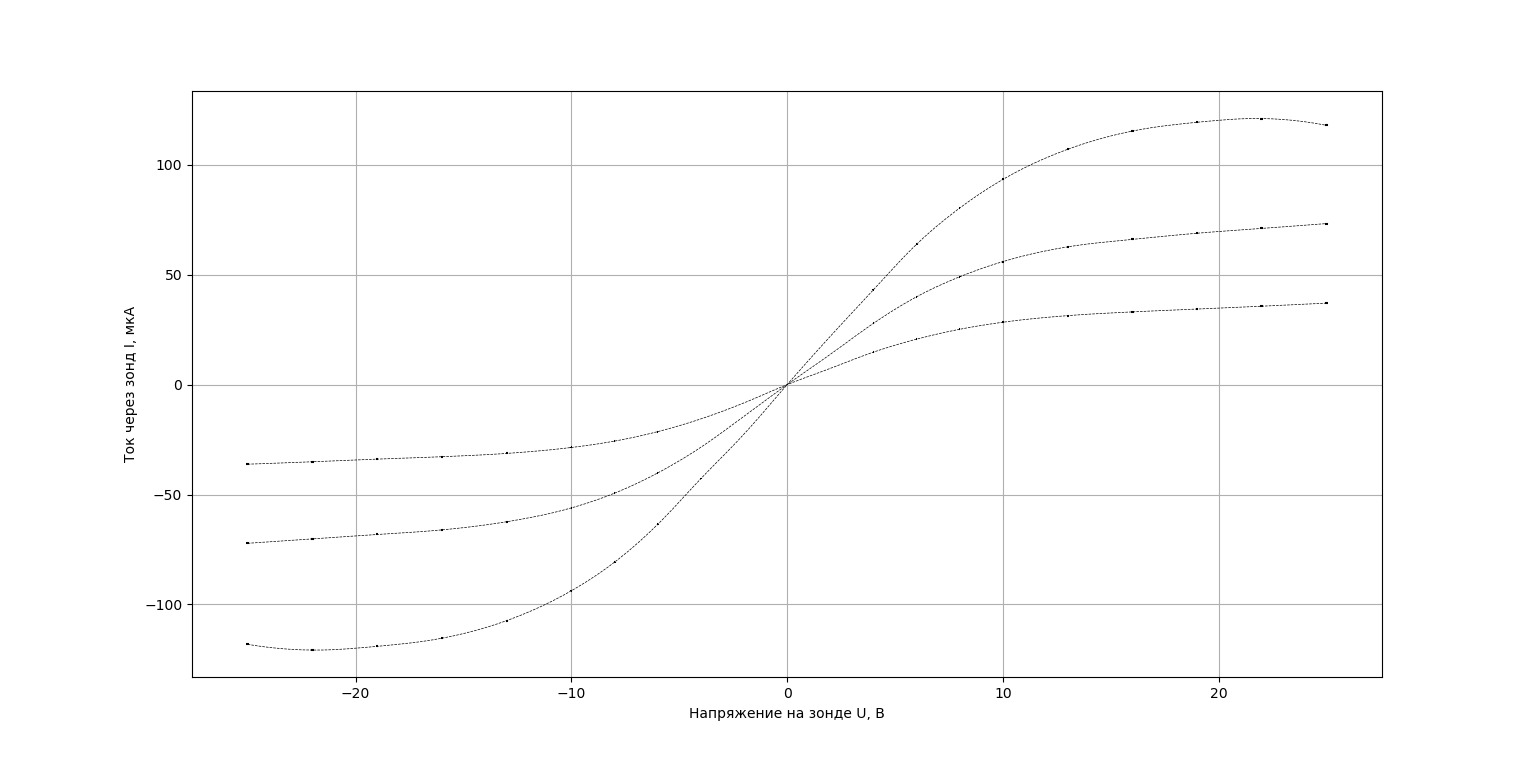
\includegraphics[scale=0.30]{zoondz}
	\caption{Семейство зондовых характеристик $I_{\text{з}}\left(U_{\text{з}}\right)$ при токах через разряд $I_{\text{р}}=1,5~\text{мА},\ 3,0~\text{мА}\ \text{и}\ 5,0~\text{мА}$. Сглаживающие кривые проведены с помощью кубических сплайнов} \label{zoondz}
\end{figure}

Определим концентрацию электронов $n_e$, считая её равной концентрации ионов $n_i$ и используя формулу Бома:\[I_{i\text{н}}=0,4n_eeS\sqrt{\frac{2kT_e}{m_i}}\implies n_e=\frac{2,5I_{i\text{н}}}{eS}\sqrt{\frac{m_i}{2kT_e}}=\frac{2,5I_{i\text{н}}}{\pi dle}\sqrt{\frac{m_i}{\Delta U}},\]где $S=\pi dl$ -- площадь поверхности зонда, а $m_i=22\cdot1,66\cdot10^{-27}~\text{кг}$ -- масса иона неона. Посчитанные по формуле значения $n_e$ тоже занесём в таблицу \Ref{Electrons}.

Зная концентрацию электронов в плазме, несложно найти их плазменную частоту колебаний по формуле\[\omega_p=\sqrt{\frac{4\pi n_ee^2}{m_e}}\ \left[\text{СГС}\right]=5,6\cdot10^4\sqrt{n_e}\ \left[\text{СГС}\right]=5,6\cdot10^1\sqrt{n_e}\ \left[\text{СИ}\right].\]Результаты также занесём в таблицу \Ref{Electrons}. Заметим, что при падении на эту плазму электромагнитного излучения через неё пройдут волны с частотами, \textit{превышающими} $\omega_p$.

Рассчитаем теперь электронную полряизационную длину $r_{De}$. Используем формулу\[r_{De}=\sqrt{\frac{kT_e}{4\pi n_ee^2}}=\frac{1}{\omega_p}\sqrt{\frac{e\Delta U}{2m_e}}.\]Занесём результаты в таблицу \Ref{Electrons}.

По формуле\[r_{D}=\sqrt{\frac{kT_i}{4\pi n_ee^2}}=\frac{1}{\omega_p}\sqrt{\frac{kT_i}{m_e}},\]где $T_i\approx300~\text{К}$, найдём дебаевский радиус. Занесём результаты в таблицу \Ref{Electrons}. Из полученных значений ($10^{-4}\ldots10^{-3}~\text{см}$) очевидно, что плазму \textit{можно считать квазинейтральной} при всех используемых в работе токах разряда.

Оценим теперь среднее число ионов $N_D$ в дебаевской сфере:\[N_D=\frac{4\pi}{3}r_D^3n_i.\]Занесём результаты в таблицу \Ref{Electrons}. Из полученных значений ($N_D\gg1$) делаем вывод, что \textit{плазма является идеальной}.

Давление в плазме приближённо равно $P\approx2~\text{торр}=266,6~\text{Па}$, тогда можно найти полную концентрацию как $n=\frac{P}{kT_i}=6,44\cdot10^{22}$. Степень ионизации плазмы равна\[\alpha=\frac{n_i}{n},\]посчитанные по этой формуле значения занесём в таблицу \Ref{Electrons}.

Также занесём в таблицу дифференциальное сопротивление ВАХ разряда при соответствующих значениях $I_{\text{р}}$.

\begin{table}[h]
	\centering
	\caption{Параметры плазмы} \label{Electrons}
	\begin{tabular}{|c|c|c|c|}
		\hline
		$I_{\text{р}}$, мА & $1,50\pm0,02$ & $3,00\pm0,02$ & $5,00\pm0,02$ \\ \hline
		$R_{\text{диф}},\ \text{к}\Omega$ & $5,00\pm0,15$ & $1,25\pm0,07$ & $0,26\pm0,01$ \\ \hline
		$T_e,\ 10^4~\text{К}$ & $4,00\pm0,03$ & $4,54\pm0,04$ & $5,89\pm0,05$ \\ \hline
		$n_e,\ 10^{16}~\text{м}^{-3}$ & $2,29\pm0,02$ & $4,50\pm0,05$ & $7,77\pm0,08$ \\ \hline
		$\omega_p,\ 10^9\frac{\text{рад}}{\text{с}}$ & $8,47\pm0,02$ & $11,88\pm0,03$ & $15,60\pm0,04$ \\ \hline
		$r_{De}$, мкм & $91,9\pm0,5$ & $69,8\pm0,4$ & $60,6\pm0,3$ \\ \hline
		$r_{D}$, мкм & $7,96\pm0,02$ & $5,68\pm0,02$ & $4,32\pm0,01$ \\ \hline
		$N_D$ & $48,4\pm0,2$ & $34,5\pm0,1$ & $26,3\pm0,1$ \\ \hline
		$\alpha,\ 10^{-7}$ & $3,56\pm0,02$ & $6,99\pm0,04$ & $12,06\pm0,06$ \\ \hline
	\end{tabular}
\end{table}

Построим теперь графики зависимостей электронной температуры $T_e(I_{\text{р}})$ и концентрации $n_e(I_{\text{р}})$ от тока разряда. Графики приведены на рисунках \Ref{temp} \Ref{conc}.

\begin{figure}[h]
	\centering
	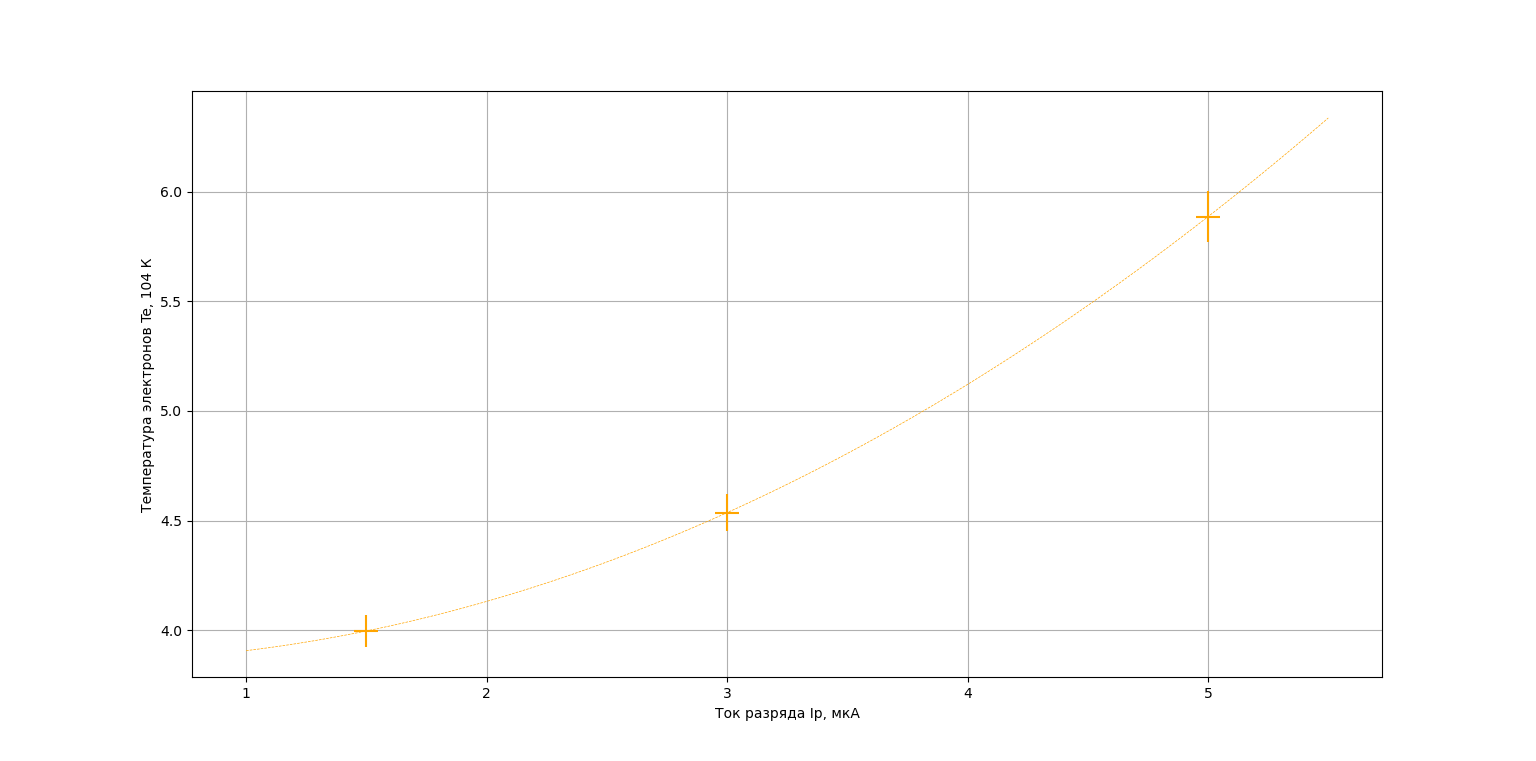
\includegraphics[scale=0.3]{temp}
	\caption{Зависимость температуры электронов $T_e$ от тока разряда $I_{\text{р}}$. Сглаживающая кривая проведена с помощью аппроксимации экспериментальных точек зависимостью $y=a+cx^2$} \label{temp}
	\centering
	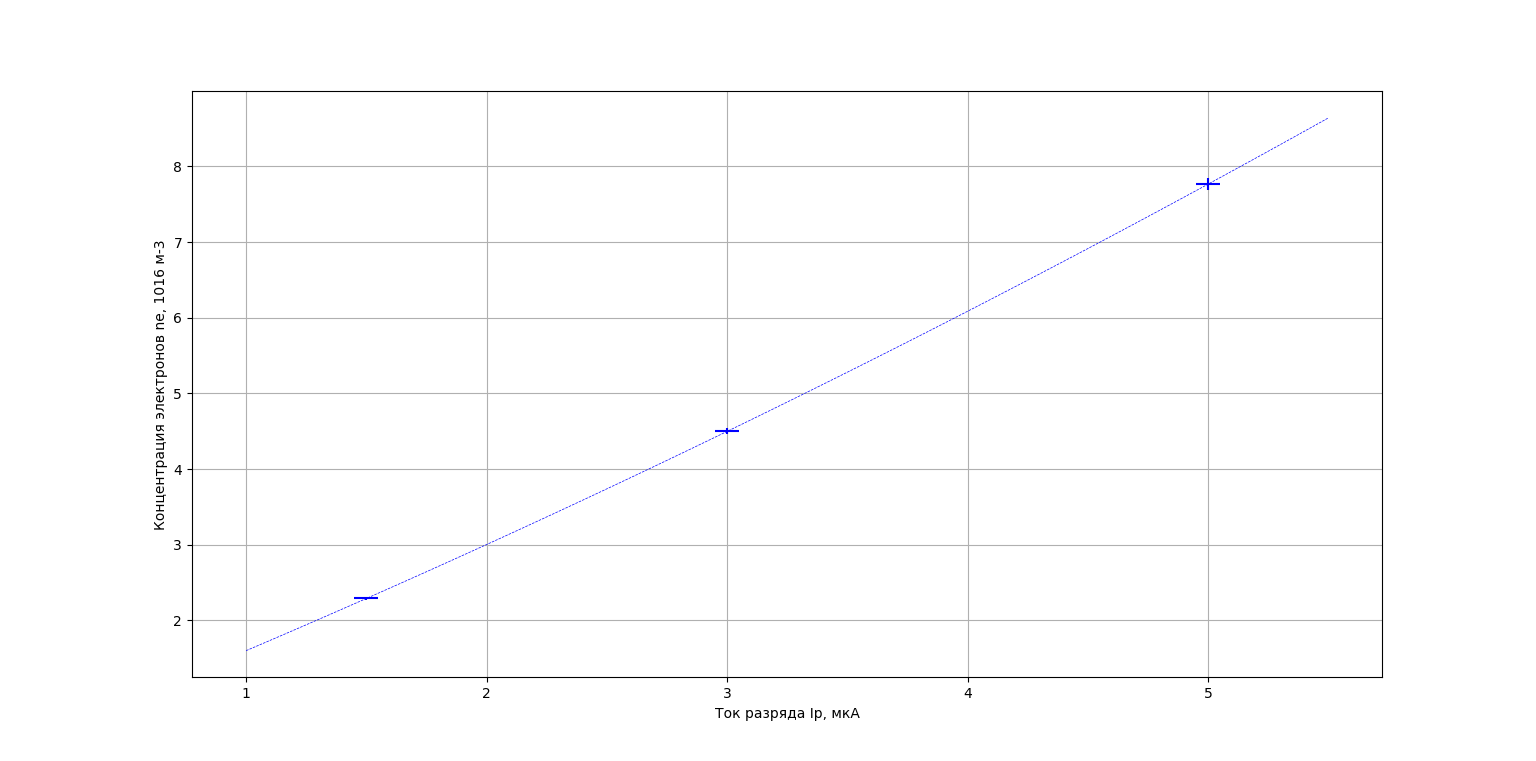
\includegraphics[scale=0.30]{conc}
	\caption{Зависимость концентрации электронов $n_e$ от тока разряда $I_{\text{р}}$. Прямая проведена по МНК} \label{conc}
\end{figure}

\section*{Вывод}

В данной работе были изучены вольт-амперная характеристика тлеющего разряда и свойства плазмы методом зондовых характеристик.

В первой части работы были проведены измерения ВАХ разряда, результат успешно сопоставлен участку, соответствующему тлеющему разряду на характерной ВАХ (см. рисунок \Ref{Characteristic}).

Во второй части работы были измерены зондовых характеристики плазмы при различных токах разряда. Полученные данные были обработаны, с их помощью было проведено исследование основных параметров плазмы -- температуры и концентрации ионов (см. таблицу \Ref{Electrons}).

В этой же части работы сделан вывод об \textit{идеальности} и \textit{квазинейтральности} плазмы во всём рабочем диапазоне.

Построены графики зависимости температуры плазмы и концентрации ионов в ней от тока разряда. Видим, что концентрация с хорошей точностью линейно растёт с увеличеснием тока, в то время как температура растёт нелинейно (к слову, полученные для температуры точки с хорошей точностью ложатся на параболу $y=3,86+0,09x^2$ с вершиной в непосредственной близости от начала координат, что говорит о возможной кадратичсной зависимости температуры электронов от тока разряда).

Относительноневысокие погрешности полученных значений говорят о точности методов, корректности работы оборудования и правильности проведения эксперимента.

\section{Приложение. Вольт-амперная характеричстика разряда в неоне}

\begin{figure}[h]
	\centering
	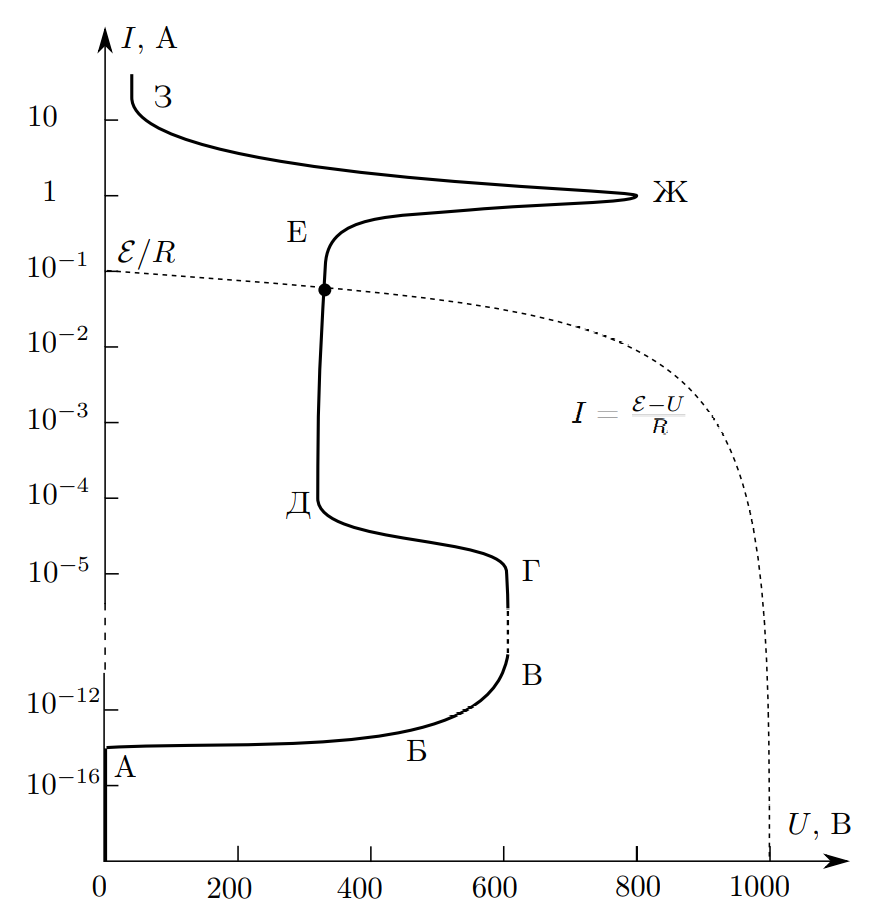
\includegraphics[scale=0.45]{Characteristic}
	\caption{Вольт-амперная характеристика разряда в неоне} \label{Characteristic}
\end{figure}

\end{document}
